\documentclass[a4paper,11pt]{article}
\usepackage[english]{babel} 
\usepackage[pdftex]{graphicx}     
\usepackage[hmargin=2cm,vmargin=2.5cm]{geometry} 
\usepackage{comment} 
\graphicspath{{.}{./images/}}
\newcommand{\degree}{\ensuremath{^\circ}}
 
\usepackage{color}
 \usepackage{here}
 l
\newcommand{\todo}[1]{{\small\color{red}[#1]}}

\usepackage{graphicx}
\begin{document}

\section{Extensions and future work}

The work presented in this paper has the advantage of being embedded into the Nao robot. The use of the Nao text to speech, speech recognition, sensing and acting capabilities makes the system easy to setup from any computer that hold the python naoqi.

However we reached some of the limits of the Nao abilities, especially when it comes to detect behaviors of users interacting with the robot. Gesture recognition, gaze traking or multiple interlocutors detection are skills far behond the embedded hardware and software of the Nao.

In order to enable more advanced interaction, we have started to devellop kinect based tools that enable to gather more precise informations from the user at the cost of an additional external device.

This section explain how it could be used to enhance the interaction with the Nao robot and describe our current implementation of Nao teleoperating system. 

\subsection{Microsoft Kinect}

Microsoft Kinect \cite{leyvand2011kinect} is an inexpensive non-invasive technology which by the means of a standard camera associated to a depth sensor is able to determinate the location of particular body joints in a 3D space. Figure \ref{KinectJoint} shows the name and body position of those joints. Recently Microsoft has released a new version of their software development kit (Kinect SDK 1.5) which, in addition of the skeleton tracking, provide support for face position and orientation tracking as well as facial features detection in real time.

Experiments to validate accuracy of the Kinect have been perform  \cite{clark2012validity} and show that, for specific clinical settings, its precision is comparable to expensive multiple-camera 3D motion analysis systems.

\begin{figure}[H]
	\centering
	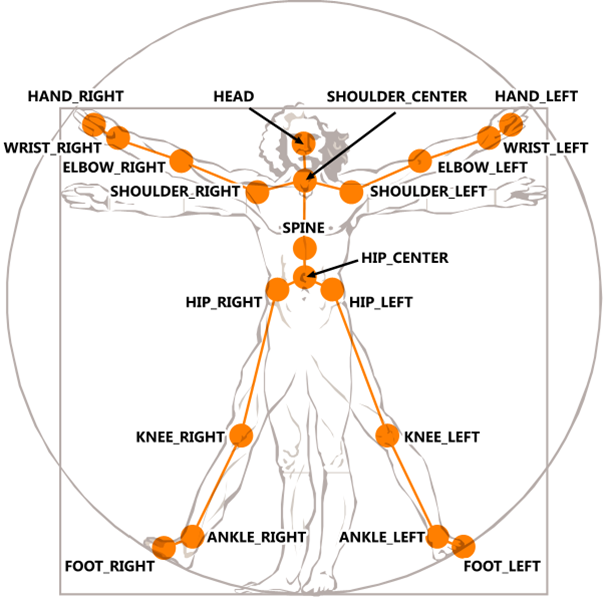
\includegraphics[width=7cm]{jointssquelette.png}
	\caption{Kinect joint name and position}
	\label{KinectJoint}
\end{figure}

\subsection{Application}
Among the different applications the Kinect could have in our system, we can make the distinction between three categories : (1) information that help the robot understanding the behavior of the user and enhance the interaction, (2) information that help us evaluating Human-Robot Interaction during user experiments and (3) tools that help us enhancing the behavior of the robot.

\subsubsection*{(1) Enhancing interaction}

The face tracking option provide head orientation and position from which can be extracted an approximation of the gaze of the user. This information can be useful to detect if the user is bored during the interaction and trigger adapted robot behaviors, such as ending the topic, asking for a new topic...
The skeleton tracking can be used to detect if a person enter or leave the room as well as the position of it in the room. That could trigger welcome and goodbye behavior as well as focus the gaze of the robot in the direction of the user. (\emph{Note that Nao robots already include a face tracking ability but is limited to close range and proper light interaction, the Kinect is more robust to ambient condition and allow for a larger interaction area.})
A gesture recognition module using data form the Kinect \cite{boulos2011web,lai2012gesture} would enable non verbal communication between the human and the robot. In our current setting, the robot is quite often using \todo{boolean??} questions that can be boring for a user to verbally reply in the long turn. The kind of recognizable gestures we could think of are nodding to say 'Yes' or 'No', arm movement to continue or stop the current topic. We could also use gesture informations to focus the robot gaze towards the hands of the user when he performs a gesture.
The multiple skeleton and face tracking Kinect abilities can even extend those option in a multi-users setting.
\subsubsection*{(2) Tracking user behaviors}

Similar informations can be use to track the user behavior during an interaction in order to get quantitate measurements of the gaze of the user, the user restlessness, the talking position...

\subsubsection*{(3) Enhancing the behavior of the robot}

Using the Kinect, one could also think of tele-operating the Nao robot, meaning that the gesture of a human standing in front of a Kinect is mapped to the body of the robot. This would decrease the amount of work needed to develop gestures for the robot. Instead of blind trial and error session using a graphical representation of the joint evolution in time, one could directly record a gesture by 'demonstrating' it to the robot. \cite{beck2010towards} investigates the creation of an affect space for the generation of emotional body language to be displayed by robots, in their case a Nao robot. The body posture where generated by the mean of motion capture data. This work focuses on static posture but can be extended to dynamic gesturing.

Finally, tele-operating the robot would make easier Wizard-of-Oz experiments where the robot gestures are remotely operated by an expert while a user experiment is running. \todo{citation}

\subsection{Teleoperating Nao upper body using the Kinect}

Microsoft Kinect is providing joint positions in a three dimensional space relative to the center of the sensor while the Nao joints are angle based controlled as describe in figure \ref{NaoJoint}. In order to teleoperate the robot we need to extract useful angle values from the joint positions as well as to filter out the noise in the data received by the Kinect. In this chapter we will refer to the name of the joints and angles as respectively referenced in the Kinect SDK (figure \ref{KinectJoint}) and in the Nao documentation (figure \ref{NaoJoint}).

\begin{figure}[H]
	\centering
	\begin{minipage}[c]{.46\linewidth}
		\centering
		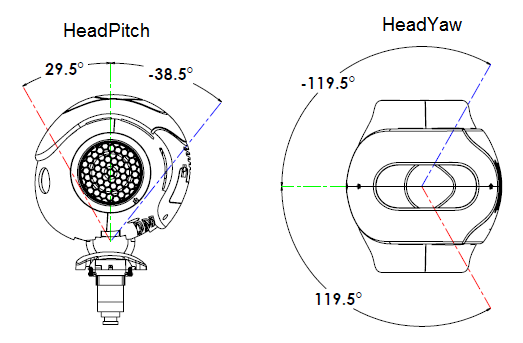
\includegraphics[width=6cm]{hardware_headjoint.png}
	\end{minipage}
	\begin{minipage}[c]{.46\linewidth}
		\centering
		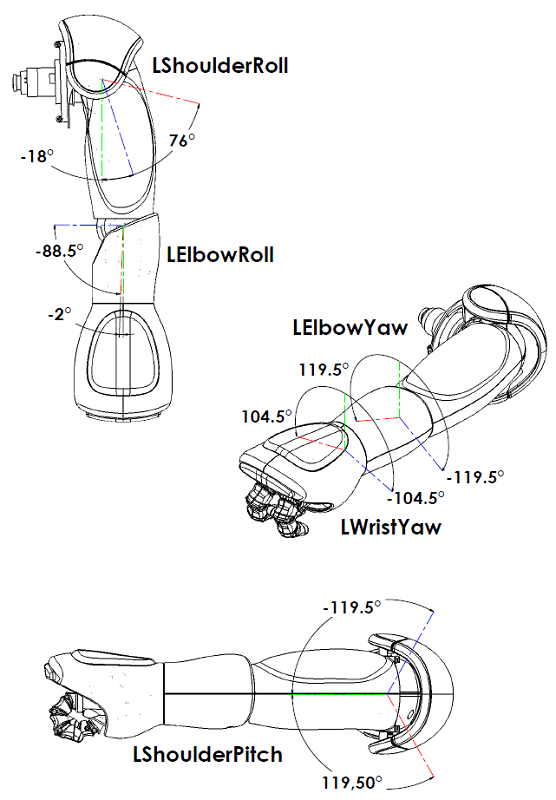
\includegraphics[width=6cm]{hardware_larmjoint.png}
	\end{minipage}
	\caption{Nao joint name, range and position}
	\label{NaoJoint}
\end{figure}

\subsubsection*{Extracting useful informations}

In order to map informations from the Kinect to the Nao, we need to extract the corresponding angles from the skeleton points gathered though the Kinect. Two aspects have to be considered, (1) the angle measure have to be independent to any other movement of the human and (2) angles should correspond to one degree of freedom of the robot. As gathered data are points in a three dimensional space, we have to choose the plane where points will be projected for the angle measurement. We describe next which plane and angle we chosen.

\subsubsection*{Head}

Kinect SDK 1.5 is directly providing information about the Head Pitch and Yaw therefore no more processing is needed for now.

\subsubsection*{Arm}

All example are given for the left arm. See figure \ref{kinecttonao} for a visual description.

\begin{itemize}
\item \textbf{LShoulder Pitch ($\alpha$):} Defined as the angle $\vec{HIP_L SHOULDER_L ELBOW_L}$ when projected on the plane whose normal vector is $\vec{SHOULDER_R SHOULDER_L}$. Projecting on this plane allow the measurement to be independent form the shoulder roll.

\item \textbf{LShoulder Roll ($\beta$):} Defined as the angle $\vec{SHOULDER_R SHOULDER_L ELBOW_L}$ on the plane to which they belong. Performing the measurement on the planed formed by those three point allow to cancel the effect of the shoulder pitch.

\item \textbf{LElbow Roll ($\theta$):} Defined as the angle $\vec{SHOULDER_L ELBOW_L WRIST_L}$  on the plane to which they belong. Performing the measurement on the planed formed by those three point allow to cancel the effect of the elbow yaw.


\end{itemize}

\begin{figure}[H]
	\centering
	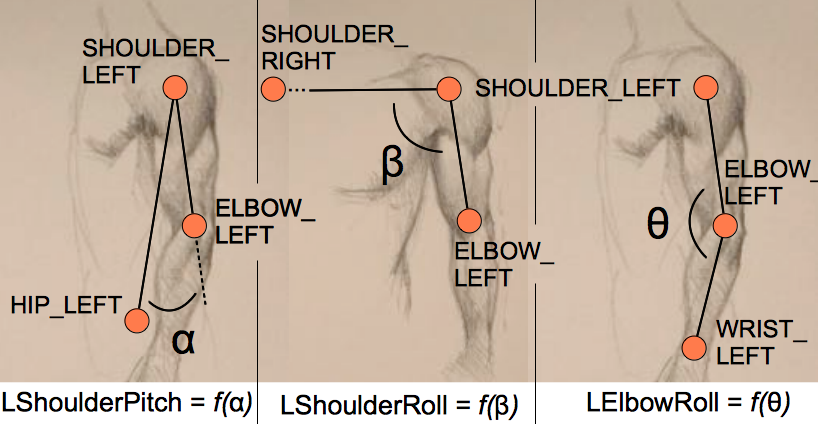
\includegraphics[width=12cm]{kinect_to_nao.png}
	\caption{Joint position to Nao angle correspondance}
	\label{kinecttonao}
\end{figure}

\subsubsection*{Mapping}

Depending on the reference and positive and negative direction, angles extracted from the Kinect data have to be shifted and/or inverted as well as min/max constrained to match with the particular Nao angle reference. 
This mapping depend on the points chosen and the positive direction defined. It can be done in different ways according to the application. In our case we are using a simple linear mapping from Kinect angle to Nao angle. A non linear mapping could also be used to have more precise movement in certain range.

\subsubsection*{Filtering}

Data from the Kinect are collected at a frequency of 30Hz \todo{to be confirmed} and are noisy. In order to provide smooth mapping from human gestures to robot movements, the noise have to be cancelled. Removing noise will add a delay between  data acquisition and actual movement on the robot.

As described in figure \ref{filter}, we are using two mean filters in a row. For every new data received from the Kinect, angles are computed as previously describe and are pushed into a \todo{rolling??} list of predefined size. Then the mean of the value in this list is used to compute the corresponding Nao angle which is pushed into a second list of predefined size. Finally the mean of this Nao angle list is used to control the robot. The choice of the buffer size is a trade-off between delay in execution and smoothing of the trajectory,  in our case the Kinect and Nao angle list are of length 10 and have been chosen by empirical test. 

In case empty or incomplete data are receive from the Kinect (person left the room, Kinect obstruction..), an empty value is pushed into the Kinect angle list. This value is not taken into account when computing the mean. This simple method allow a smooth and yet reactive filtering.

\begin{figure}[H]
	\centering
	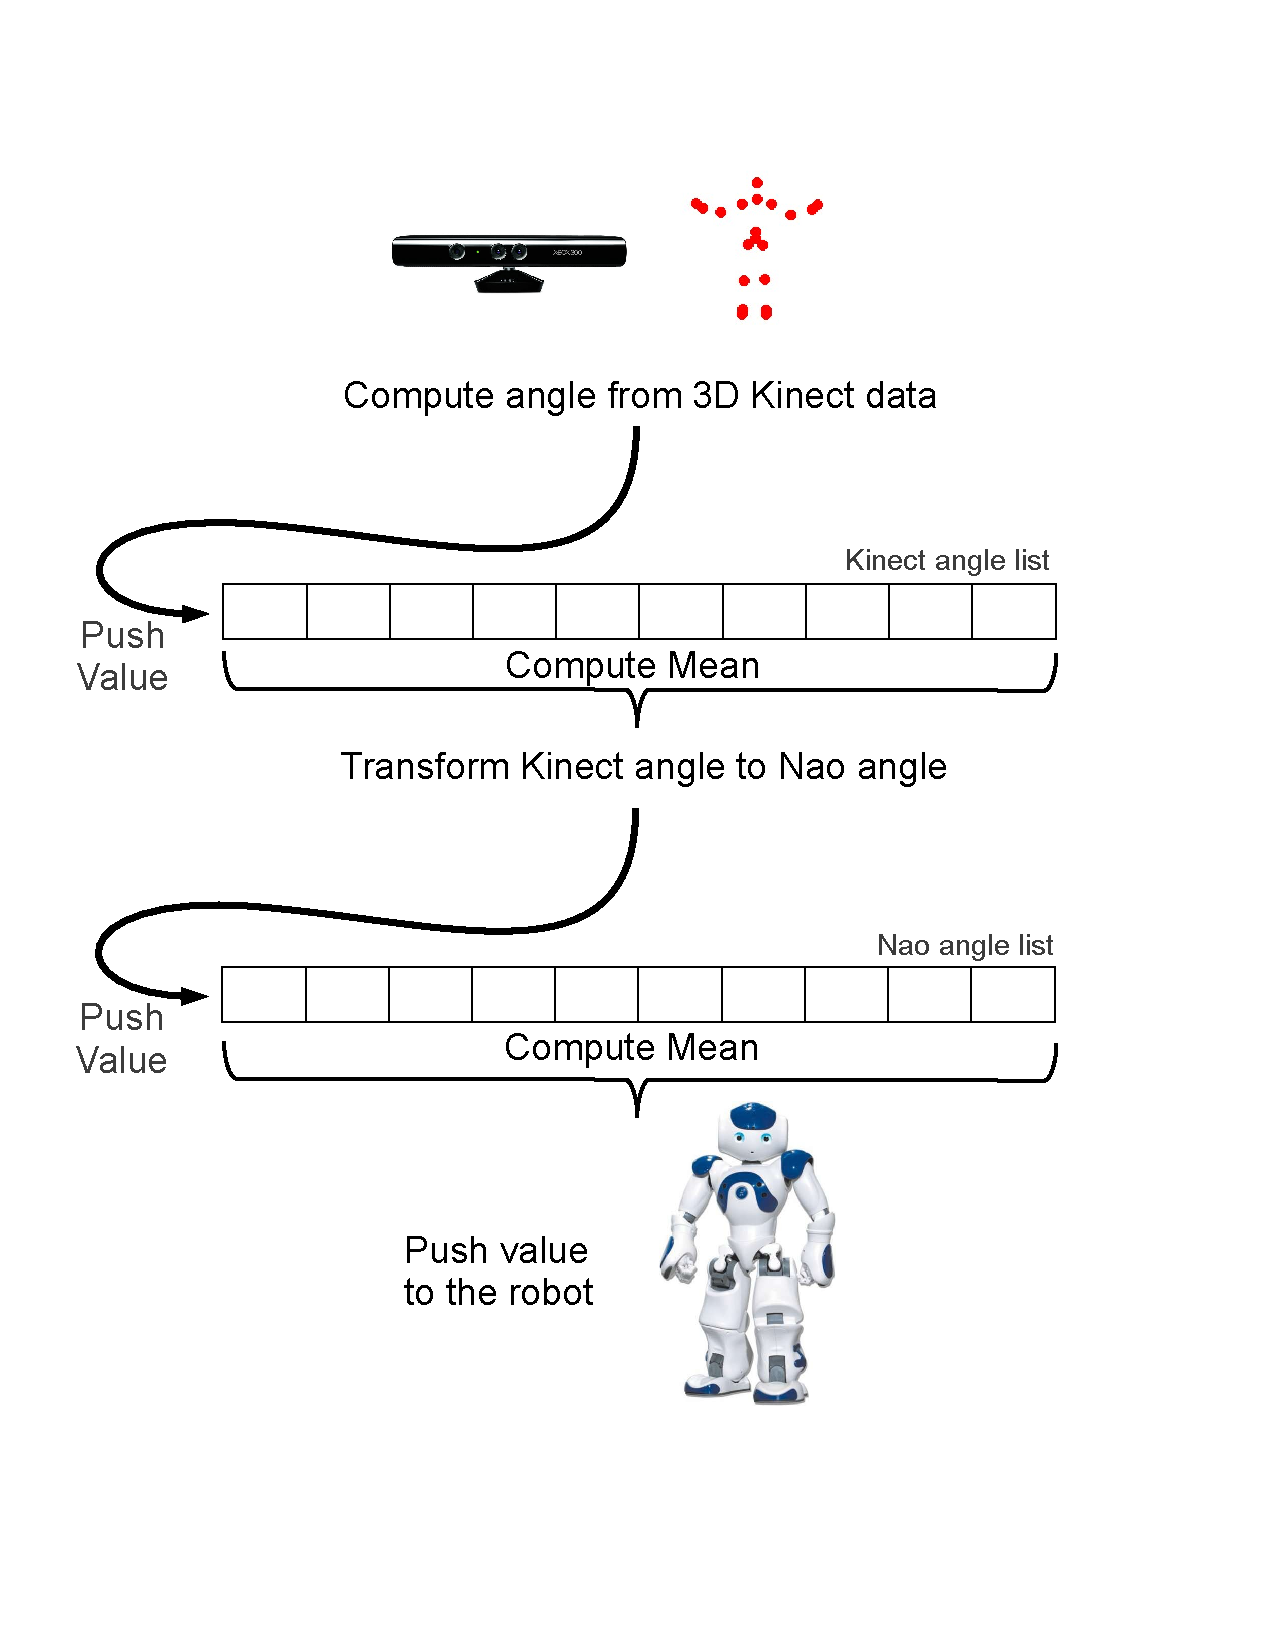
\includegraphics[width=8cm]{filter.pdf}
	\caption{Double mean filtering of the Kinect data}
	\label{filter}
\end{figure}

\todo{It could be interesting to show a graph with the recorded angle from the Kinect and after the filtering, to visualize both delay and smoothing.}

In addition to this simple filter, the Nao robot is not performing 'as fast as possible' moves but we have set the \emph{fraction\_of\_max\_speed} variable to $0.5$ \todo{to be confirmed} in the \emph{setAngles} function from Nao \emph{ALmotion} proxy. This setting avoid having the robot reaching is current goal before receiving a new one (i.e. avoid shaky movements) and have been evaluated by empirical test.

\subsection{Personal comments}

Looking again into the new Kinect SDK, I found out it also provides informations about the bone orientations which could be used to infer the missing Nao angle value that are WristYaw and ElbowYaw.

Following our discussion, I would say that there is nothing in this summary above the state of art concerning the Kinect data analysis and robot teleoperation. However and if it has never been done, using information such as head orientation as well as some dynamic gesture recognition in the system we have been developing during eNTERFACE'12 could be an interesting extension. 
There is certainly plenty of ideas we could come up with, and the limitation come from the time we can spend on it.  If our big paper is well accepted by the community, it would be interesting to propose again a project at next eNTERFACE'13 workshop, that we could develop some extensions and importantly perform user studies. But that is quite far away..

To point out a work related to gesture recognition of a Phd student from my team at INRIA, you can have a look at the abstract of his paper \cite{Mangin2012} accepted at IROS'12 (see below). That is very recent work which is much more advance than gesture recognition alone.
Here is the abstract : \textit{We present an approach, based on non-negative matrix factorization, for learning to recognize parallel combinations of initially unknown human motion primitives, associated with ambiguous sets of linguistic labels during training. In the training phase, the learner observes a human producing complex motions which are parallel combinations of initially unknown motion primitives. Each time the human shows a complex motion, he also provides high-level linguistic descriptions, consisting of a set of labels giving the name of the primitives inside the complex motion. From the observation of multimodal combinations of high-level labels with high-dimensional continuous unsegmented values representing complex motions, the learner must later on be able to recognize, through the production of the adequate set of labels, which are the motion primitives in a novel complex motion produced by a human, even if those combinations were never observed during training. We explain how this problem, as well as natural extensions, can be addressed using non-negative matrix factorization. Then, we show in an experiment in which a learner has to recognize the primitive motions of complex human dance choreographies, that this technique allows the system to infer with good performance the combinatorial structure of parallel combinations of unknown primitives.}


\bibliographystyle{plain}
\bibliography{enterface_kinect.bib}

\end{document}
